 \documentclass[12pt]{article}
\usepackage[utf8]{inputenc}
\usepackage{amsmath}
\usepackage{amssymb}
\usepackage[english]{babel}
\usepackage[margin = 1 in]{geometry}
\usepackage{wrapfig}
\usepackage{enumitem}
\usepackage{caption}
\usepackage{csquotes}
\usepackage{xcolor}
\usepackage{graphicx} 
\usepackage{subfig}

\usepackage{subfig}

\title{Project 3 - SI1336 Simulation and modelling}
\author{Raymond Wang} 
\date{November 26, 2020}
\begin{document}
\maketitle
\newpage
\section*{Project 3.1}
\subsection*{Computational time versus integration error}
In order to plot computational time against integration error for the two methods, the integration error was computed as the error of the mean of the difference between analytical and numerical values for several estimations. I.e. 
\begin{equation*}
\text{numerical} - \text{analytical},
\end{equation*}
of which the analytical value is equivalent to $\pi^5/120$. Subsequently the computational time can be measured. For the Midpoint method, computational time is dependent on the number of steps and for the Monte-Carlo estimation, the number of points. 
\begin{figure*}[ht!]
\begin{center}
   \subfloat[\label{genworkflow}]{%
      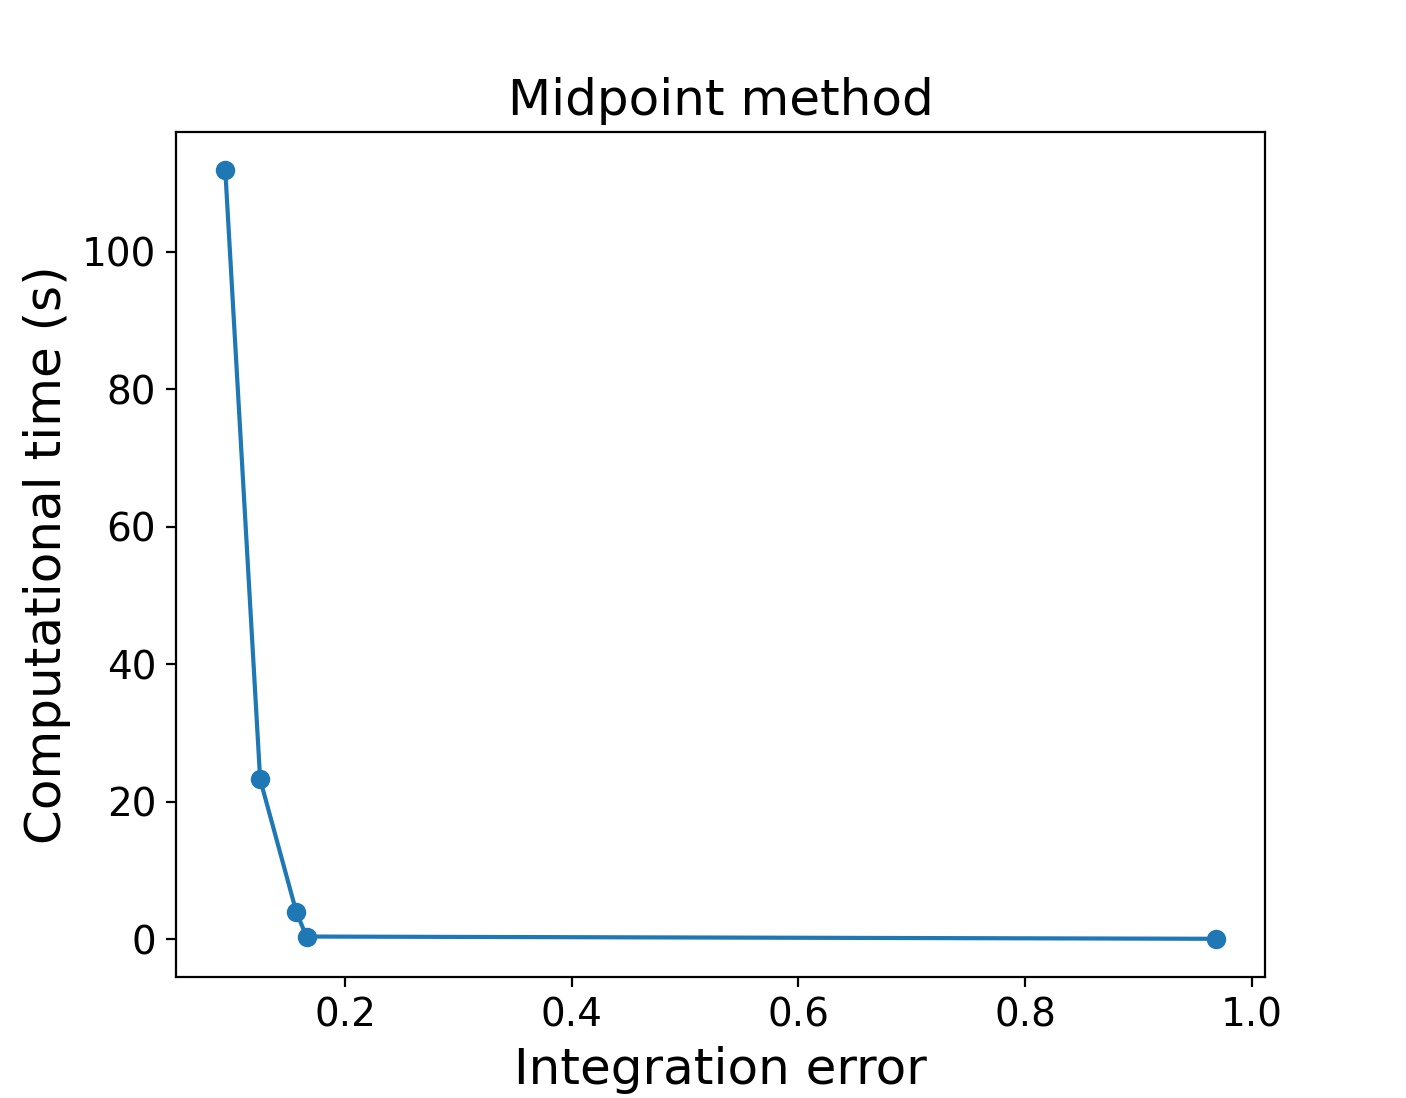
\includegraphics[width=0.45\textwidth]{Midpoint.jpg}}
   \subfloat[\label{pyramidprocess}]{%
      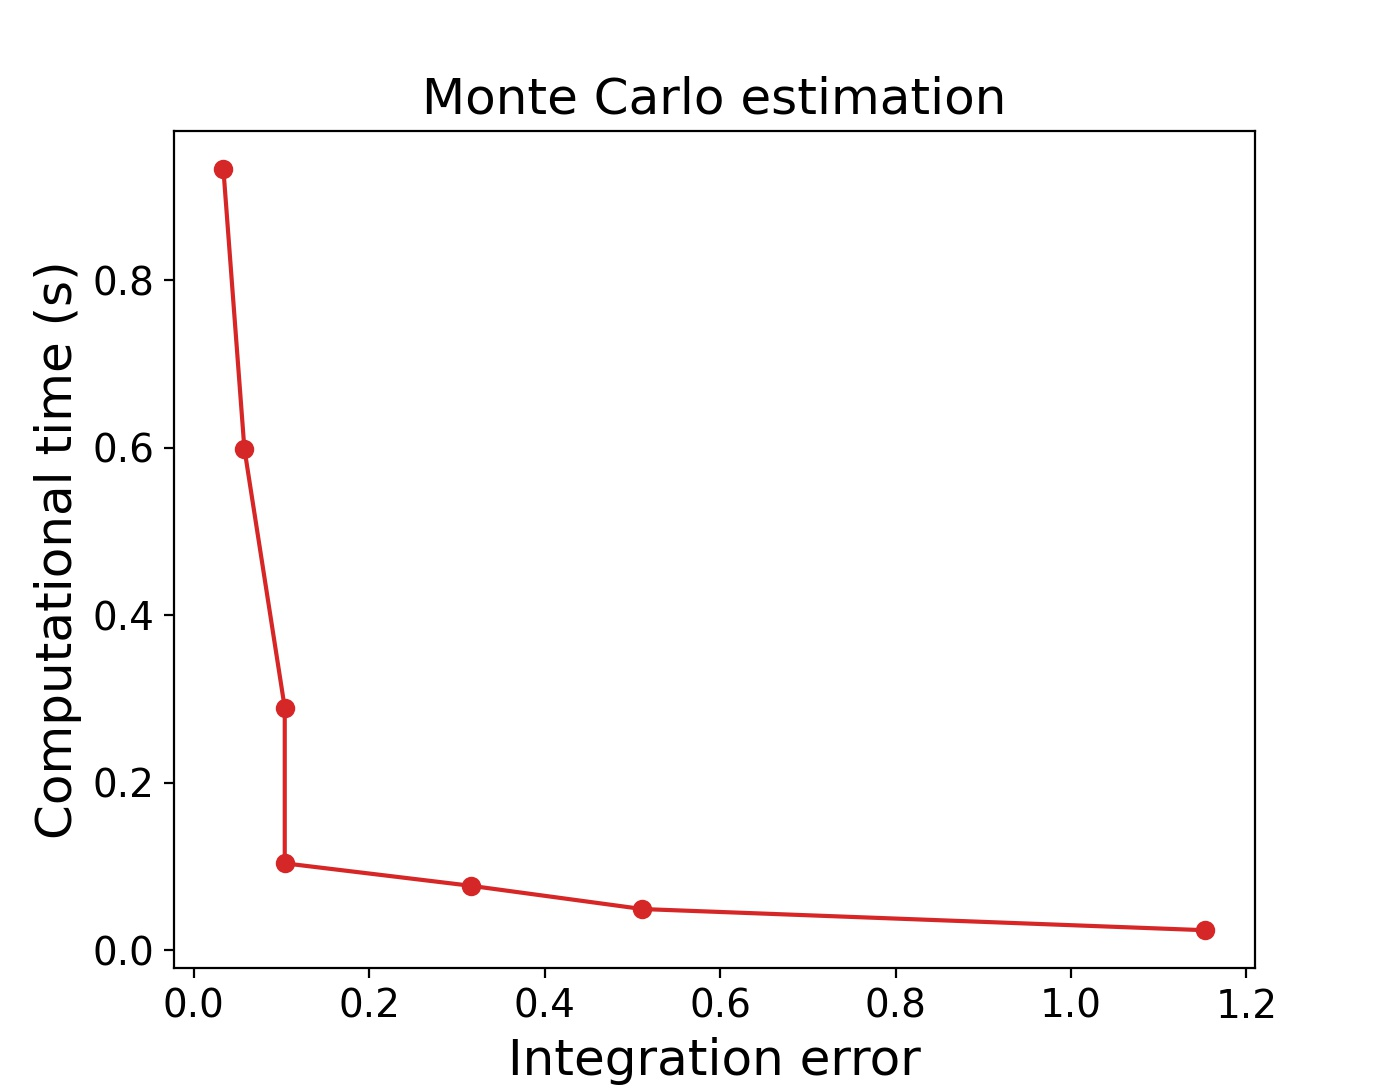
\includegraphics[ width=0.45\textwidth]{Montecarlo.jpg}}\\
   \caption{\label{workflow} (a) Midpoint method (b) Monte Carlo estimation}
\end{center}
\end{figure*}

\noindent As can be noted, this aforementioned correlation is clearly rational. For large integration errors, the difference in computational time is negligible. However, for an error within the range of 0.2, the required computational time starts increasing asymptotically. Hitherto, it can be deduced that that the Midpoint method requires a much longer computational time to attain the same quantity of error than the Monte-Carlo estimation. 
\vspace{0.3cm}

\noindent To summarize, the two methods require similar computational times to attain errors larger than 0.2. For errors smaller than 0.2, the Midpoint method necessitates much longer computational times than Monte-Carlo.

\newpage 
\section*{Project 3.2}
\subsection*{3.2a) Fluctuation in total energy for molecular motion}
A Lennard-Jones (1) potential and force (with $\sigma = 1$ and $\epsilon=1$) was implemented on a molecular simulation with 24 particles at temperature $T = 1$.
\begin{equation}
V_\text{LJ} = 4\varepsilon \left[ \left(\frac{\sigma}{r}\right)^{12} - \left(\frac{\sigma}{r}\right)^6 \right]   
\end{equation}
Upon this framework, the quality
of the integration can be deduced by monitoring the drift in the total energy for several different time steps. For
step sizes $dt = 10^{-2} - 10^{-5}$ the following energy diagrams were obtained.

\begin{figure*}[ht!]
\begin{center}
   \subfloat[\label{genworkflow}]{%
      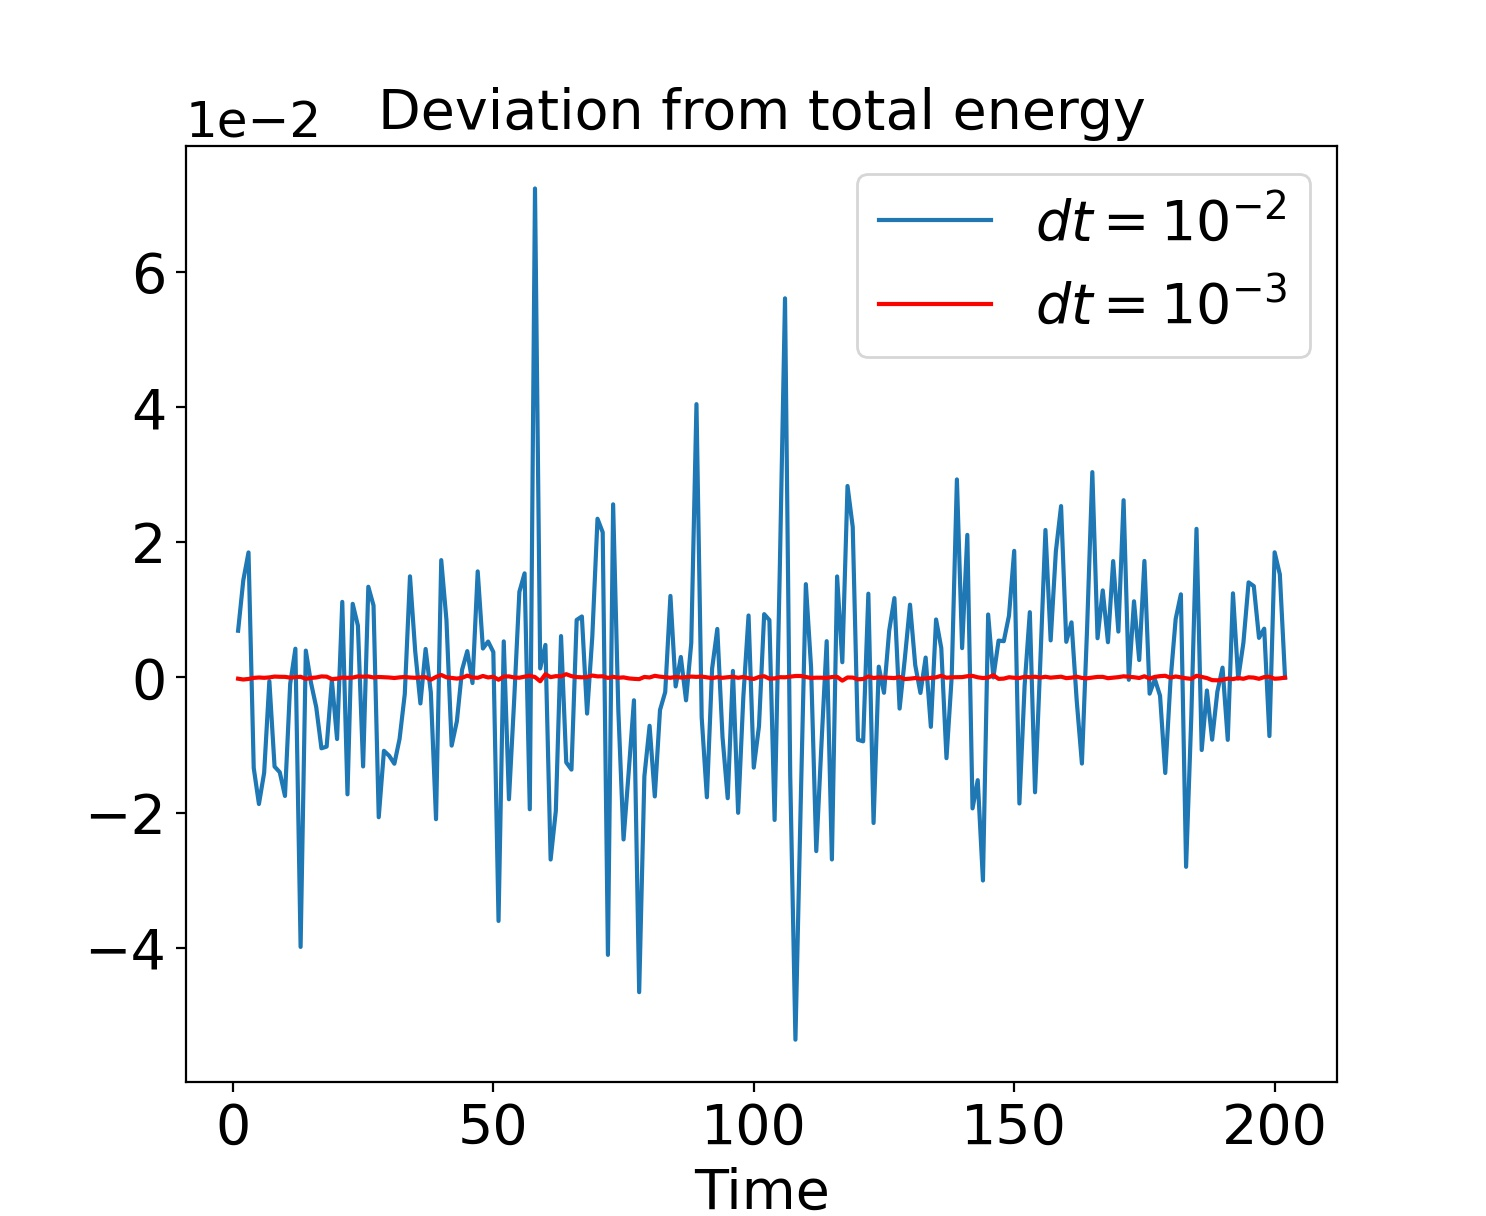
\includegraphics[width=0.33\textwidth]{Energy1.jpg}}
   \subfloat[\label{pyramidprocess}]{%
      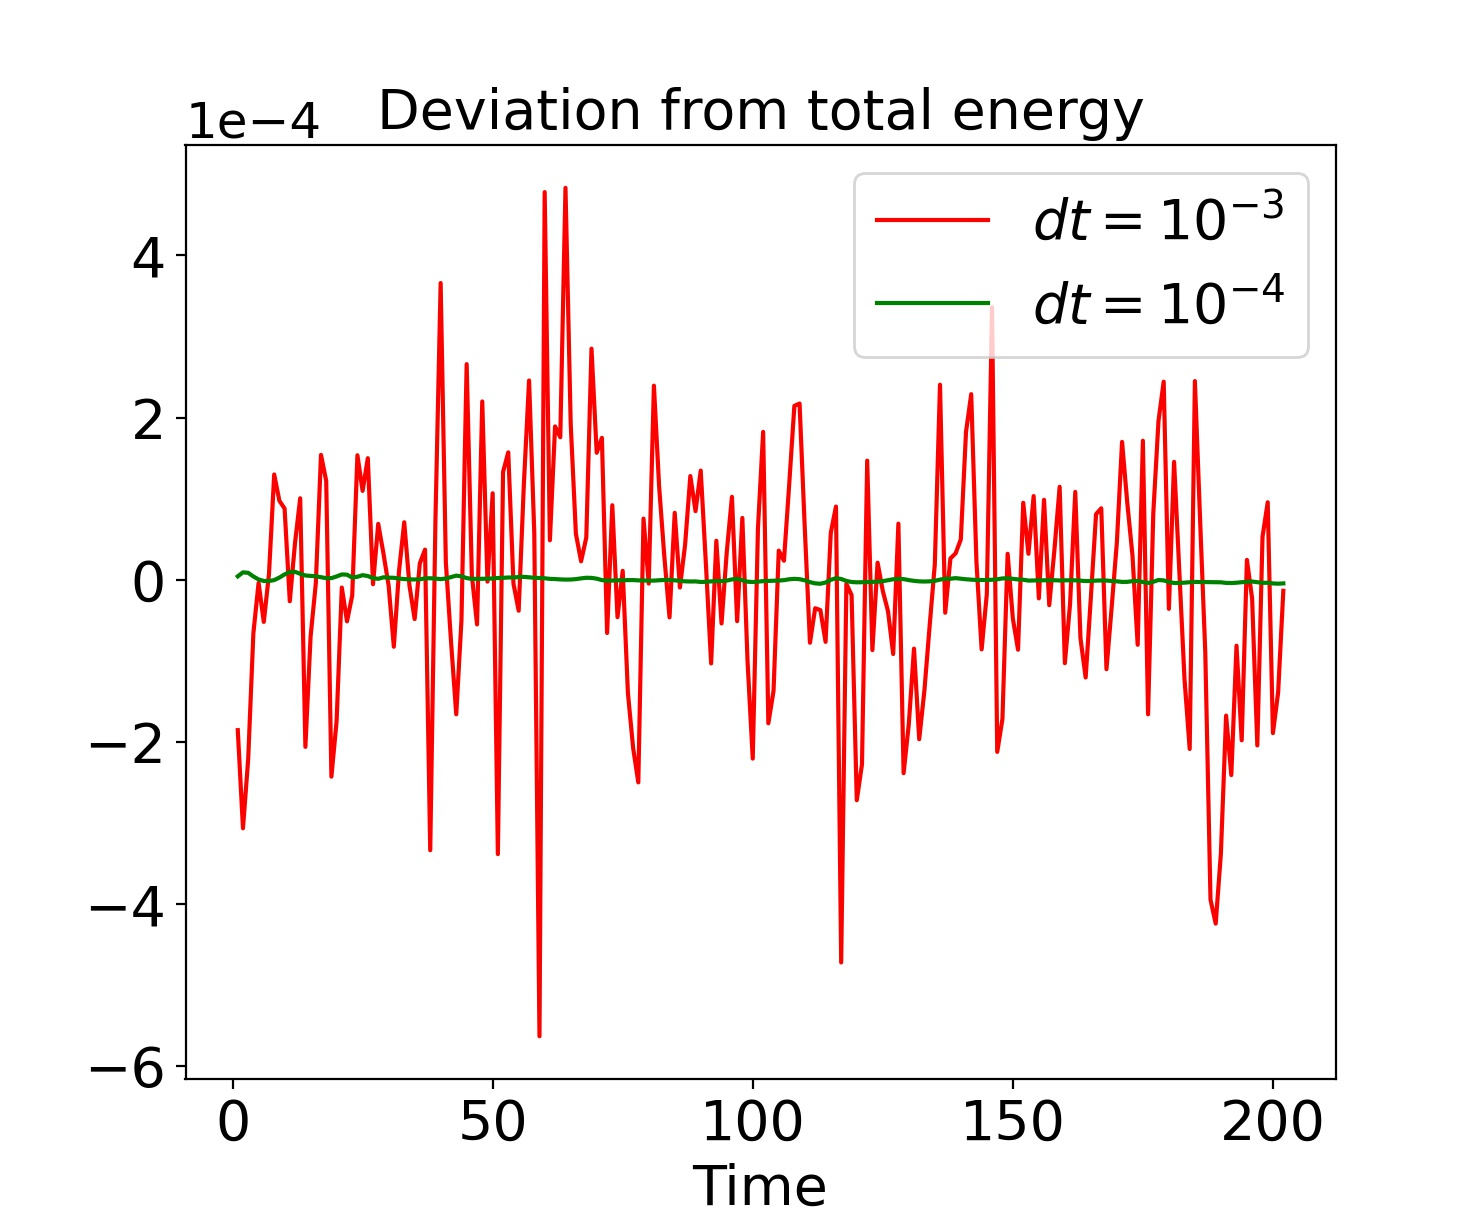
\includegraphics[ width=0.33\textwidth]{Energy2.jpg}}
   \subfloat[\label{mt-simtask}]{%
      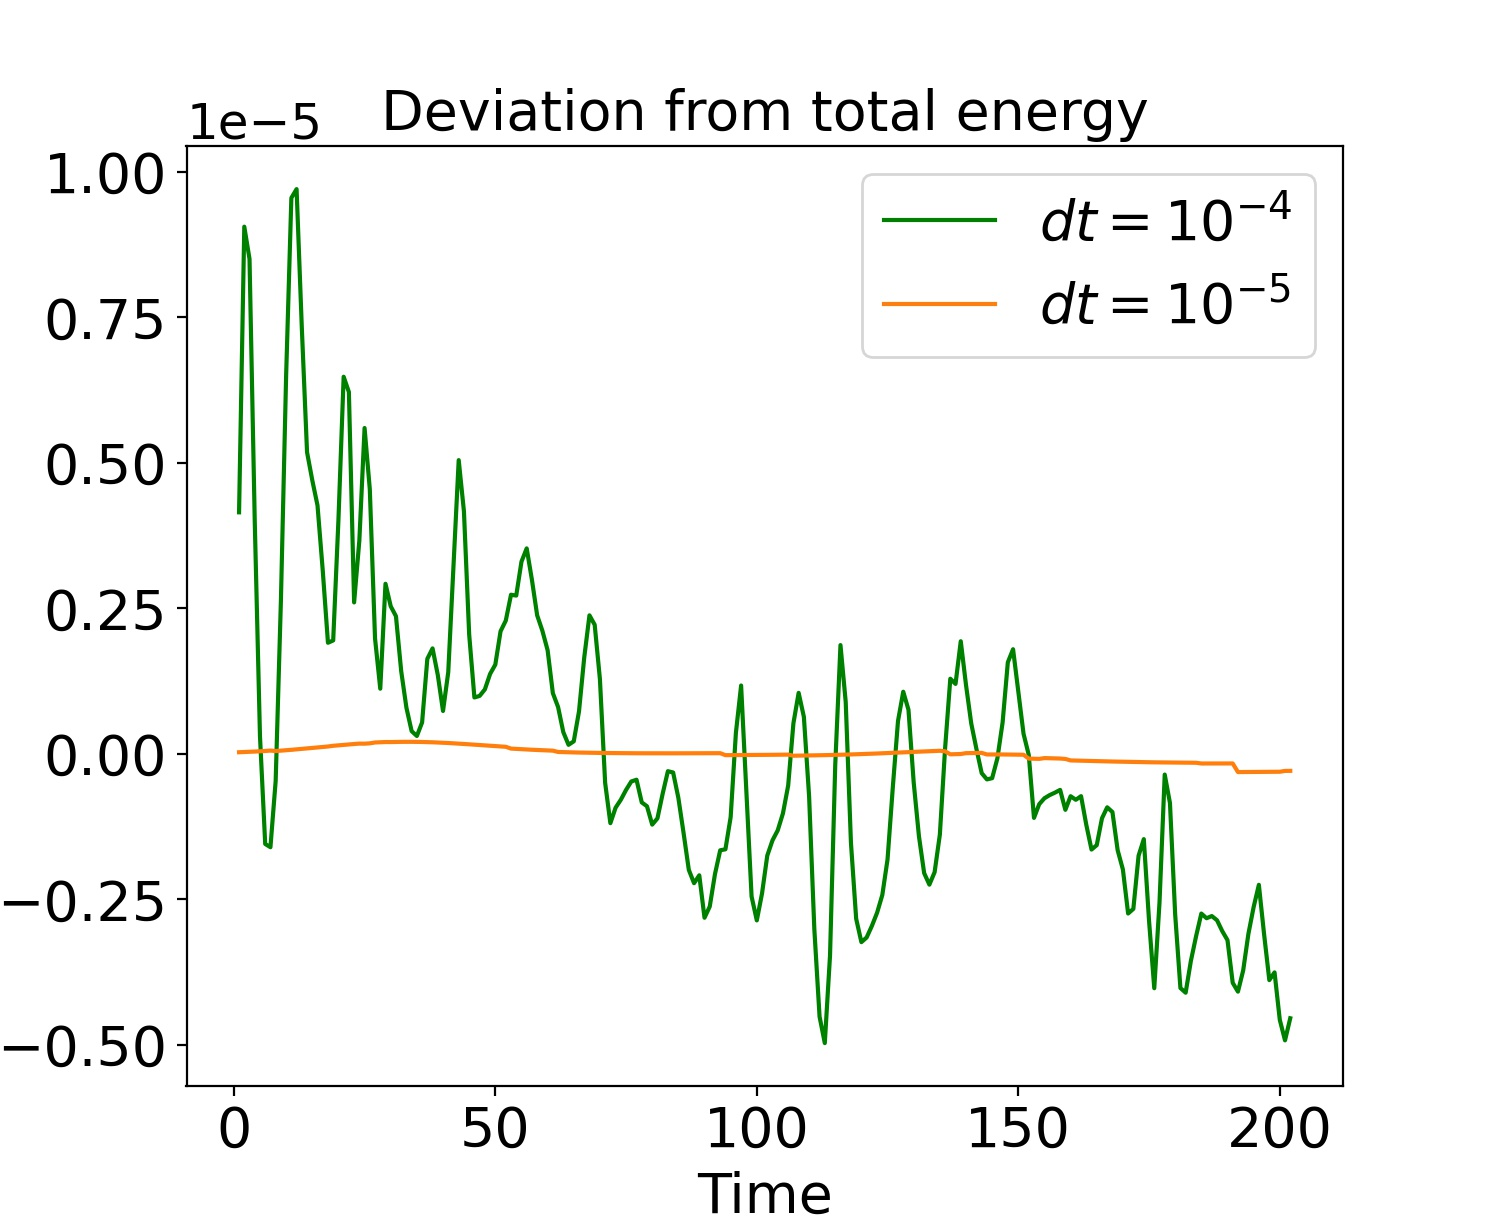
\includegraphics[width=0.33\textwidth]{Energy3.jpg}}\\
   \caption{\label{workflow} (a) $dt = 10^{-2}$ \& $10^{-3}$  (b) $dt = 10^{-3}$ \& $10^{-4}$ (c) $dt = 10^{-4}$ \& $10^{-5}$}
\end{center}
\end{figure*}
\noindent As can be noted, the energy preservation (quality of integration) is improved as the step size $dt$ decreases. Despite a diminishing total energy for  $dt = 10^{-4}$, this fluctuation is minuscule. For $dt = 10^{-1}$ the following diagram was obtained.
\begin{figure*}[ht!]
\begin{center}
    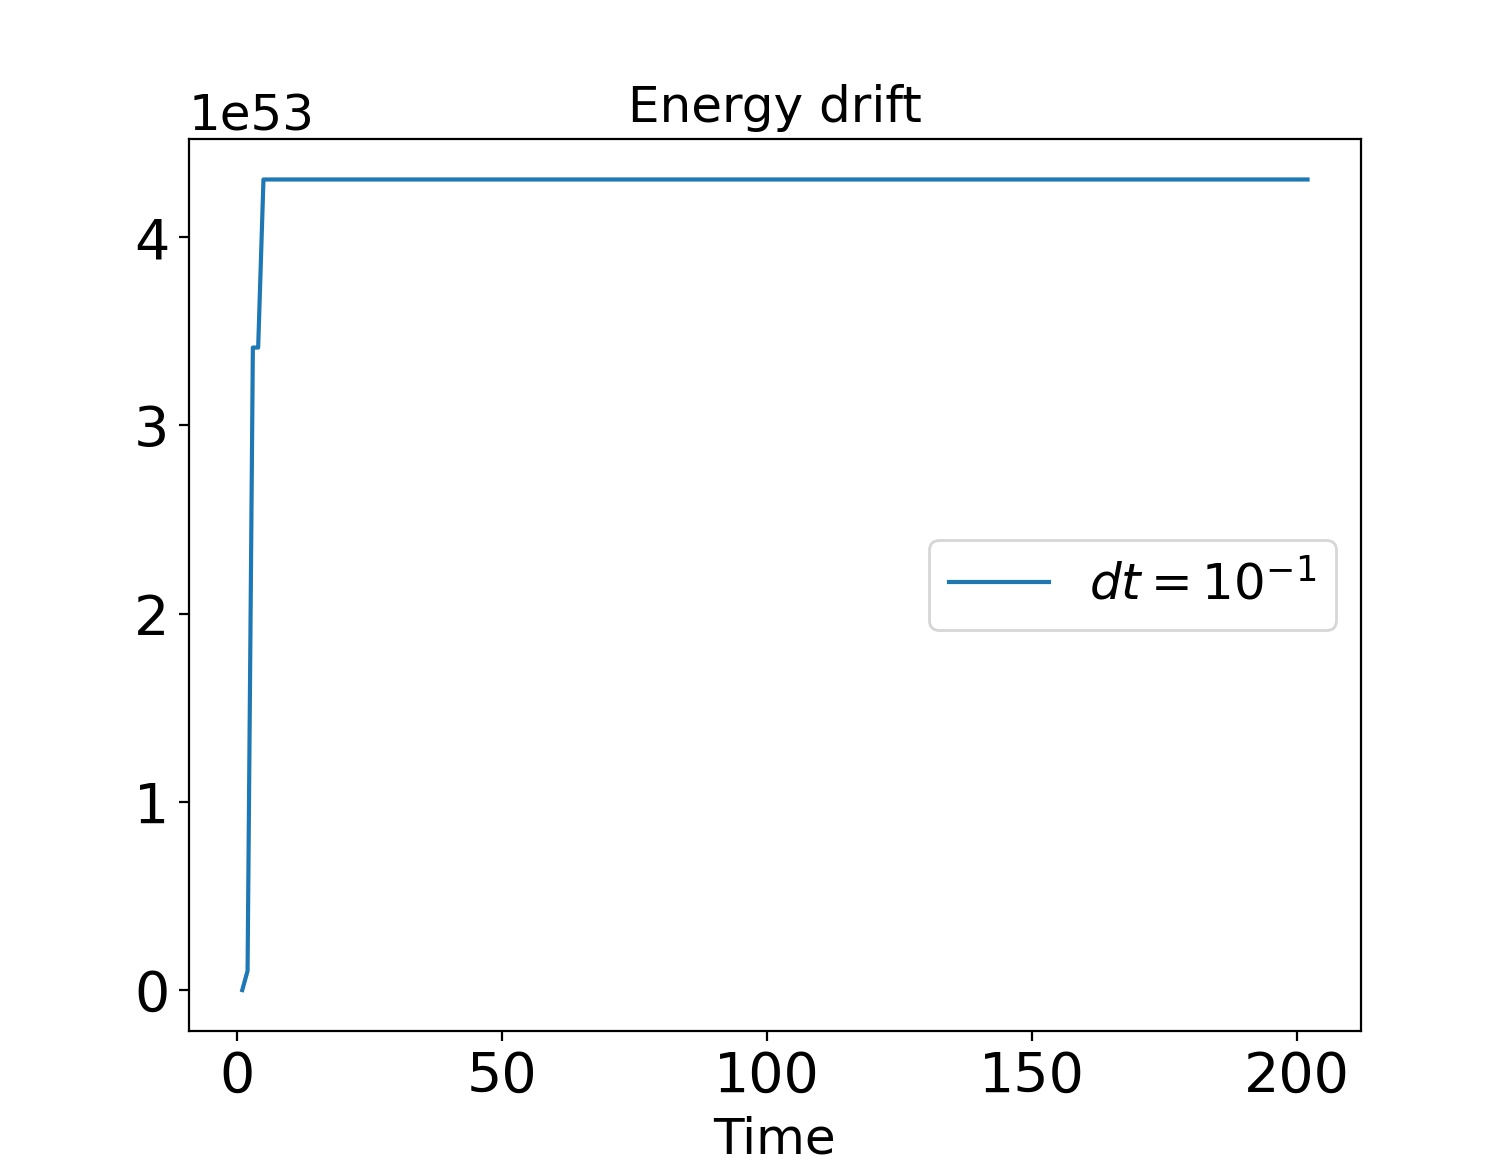
\includegraphics[width=0.38\textwidth]{Energy_0.1.jpg}
 \caption{Energy drift for $dt = 10^{-1}$}
\end{center}
\end{figure*}

\noindent As can be noted, the drift in total energy is immense, with the quality of integration thus being far more inferior compared to smaller time steps.
However, despite despite the sudden drift, the total energy is conserved for longer time frames.
\newpage 

\subsubsection*{Conclusions}
\begin{itemize}
  \item \textbf{Small dt:} Small fluctuations and better quality of integration.
  \item \textbf{Large dt:} Large fluctuations and worse quality of integration.
  \item \textbf{Best dt:} $10^{-2 } \leq dt < 10^{-1}$
\end{itemize}

\subsection*{3.2b) Fluctuation in kinetic and potential energy}
By comparing the potential and kinetic energies for temperatures $T = 1$ and 
$T = 0.2$ on the LJ-simulation, the following is to be obtained.
\begin{figure*}[ht!]
\begin{center}
   \subfloat[\label{genworkflow}]{%
      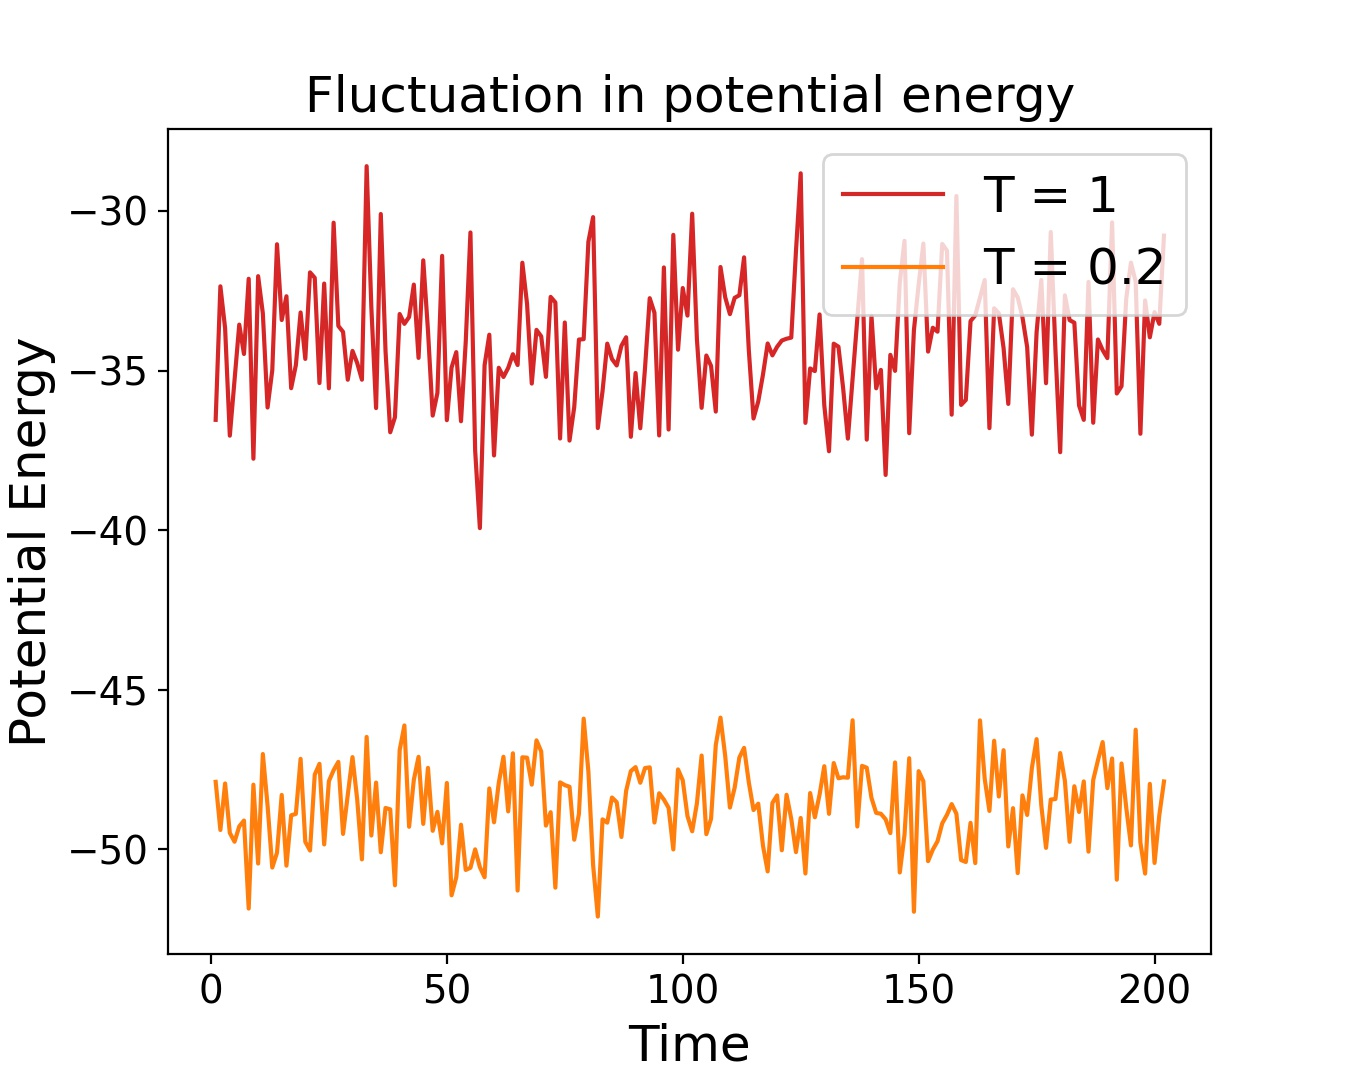
\includegraphics[width=0.45\textwidth]{Potential.jpg}}
   \subfloat[\label{pyramidprocess}]{%
      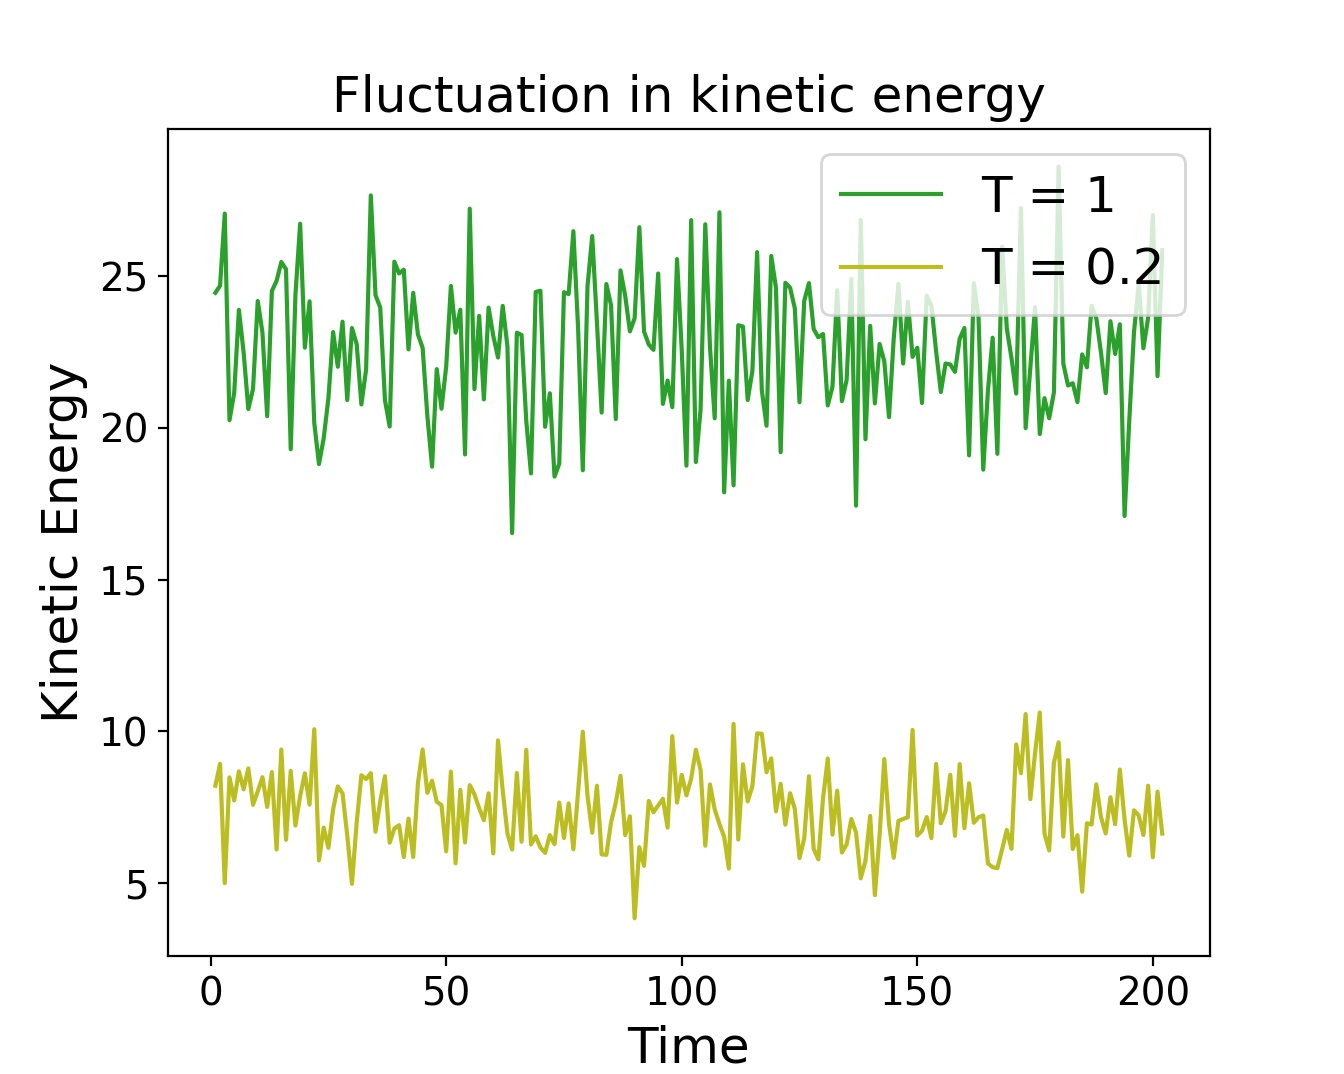
\includegraphics[ width=0.45\textwidth]{Kinetic.jpg}}\\
   \caption{\label{workflow} (a) Potential energy (b) Kinetic energy}
\end{center}
\end{figure*}

\subsubsection*{Conclusions}
\begin{itemize}
  \item \textbf{Higher T:} Larger potential and kinetic energies, and larger fluctuations
  \item \textbf{Lower T:} Smaller potential and kinetic energies, and smaller fluctuations.
\end{itemize}
Furthermore, as the fluctuations of the kinetic and potential energies show similar patterns, the variance in total energy is minuscule.


\newpage 

\subsection*{3.2c) Fluctuation in potential - Andersen thermostat}
By implementing an Andersen thermostat, thermalising particles at fixed step intervals, the following behavior for potential energy (V) is to be observed for temperatures $T = 1$ and $T = 0.2$ at long times.
\begin{figure*}[ht!]
\begin{center}
    \includegraphics[width=0.5\textwidth]{Potential_comparison.jpg}
 \caption{Potential ($V$) for $T$ = 0.2 and $T$ = 1}
\end{center}
\end{figure*}

\subsubsection*{Conclusions}
\begin{itemize}
  \item \textbf{Higher T:} Smaller fluctuations and converging for small $V$.
  \item \textbf{Lower T:} Larger fluctuations and converging for large $V$.
  \item \textbf{Collective behavior} More motion, randomized trajectories and particle distances as $T$ increases.
\end{itemize}
As for the physical interpretation, it can be concluded that $T$ is dependent on the average kinetic energy of the system. Thus, as the temperature increases, the kinetic energy increases concurrently resulting in higher particle movement and triggering a more chaotic behavior. 
The increase in in energy caused by the increase in energy also results in greater $V$, which is clearly shown in the aforementioned diagram. As kinetic and potential energies are directly correlated, the diagram clearly attest these tendencies.

\newpage 
\subsection*{3.2d) Average energy and heat capacity - Andersen thermostat}
For temperature values 
\begin{equation*}
T \in [0.2, 0.3, 0.4, 0.5, 0.6, 0.7, 0.8, 0.9, 1.0],
\end{equation*}
the (\textit{sufficiently converged}) heat capacities and average energies were recorded and plotted against time. The same number of time steps as in c) were utilized.
\begin{figure*}[ht!]
\begin{center}
    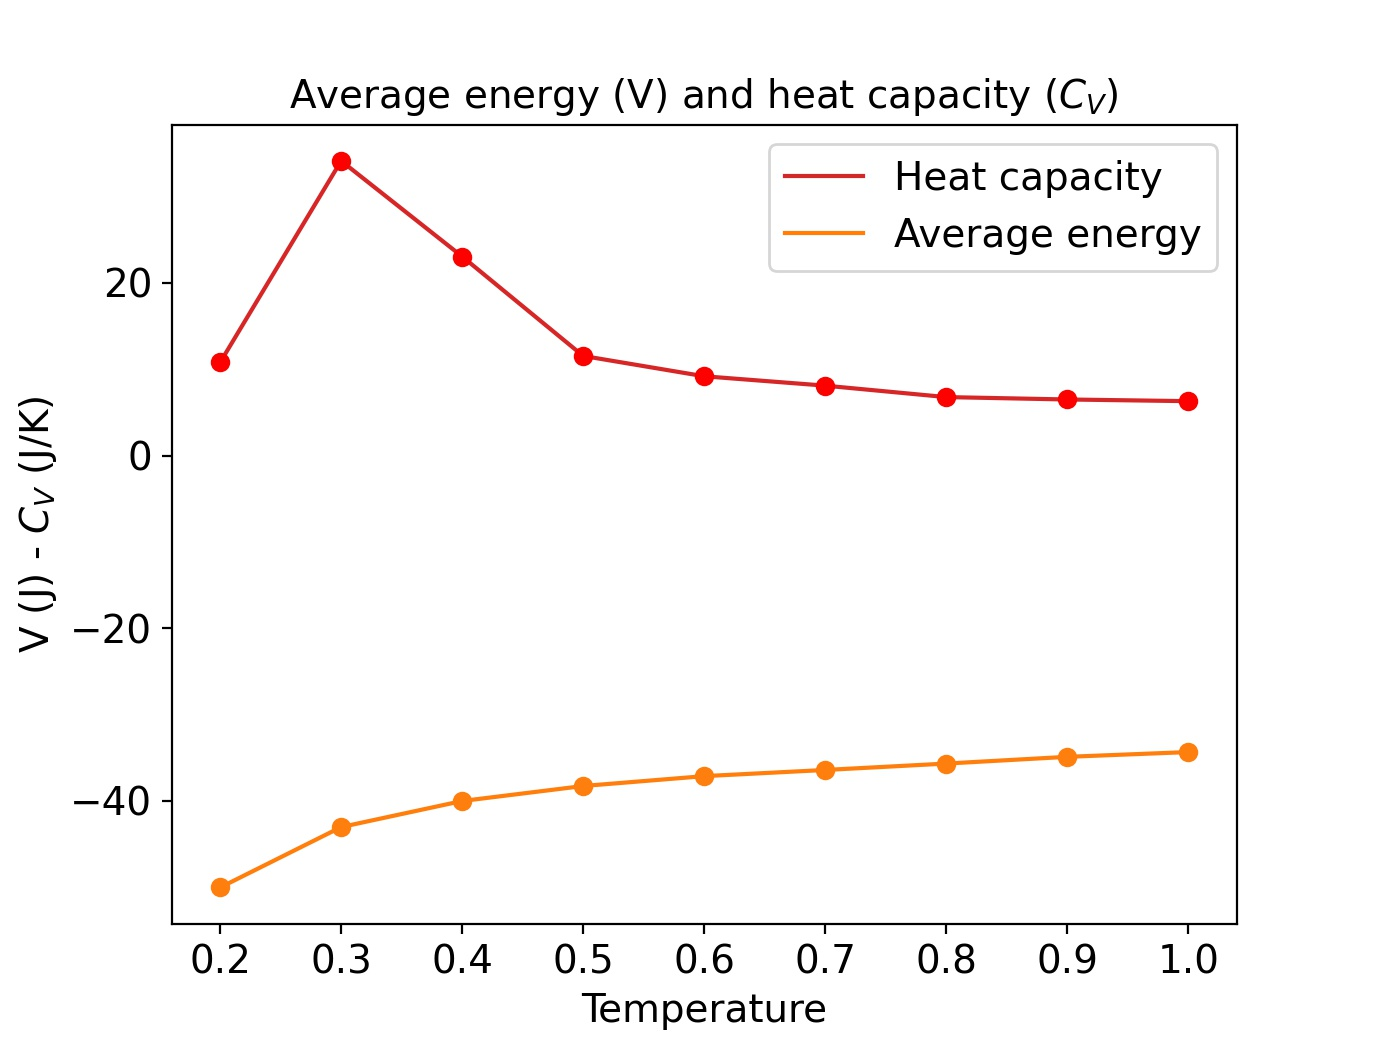
\includegraphics[width=0.5\textwidth]{Comparison.jpg}
 \caption{Average energy and heat capacity}
\end{center}
\end{figure*}

\noindent As can be noted, with larger temperatures the heat capacity decreases while converging according to $\lim_{T\to 1} V \approx 6.3$ while the average energy increases and converges according to 
$\lim_{T\to 1} C_V \approx -23$. The fact that average energy increase due to higher temperatures is trivial. However, the decrease in $C_V$ can be explained with thermodynamics.
\vspace{0.3cm}

\noindent Approximate the molecular potion as an ideal gas. As the temperature increases at constant volume, this would be considered as an isochoric process of which the heat capacity ratio $\gamma$ is increasing. This is attributed to an an increase pressure due to the rising temperatures. Using Mayer's relation, the analytic formula for heat capacity can be deduced as follows.

\begin{equation}
C_V = \cfrac{nR}{\gamma -1},
\end{equation}
where $n = $  amount of substance (mol) and $R = 8.14$ $JK^{-1}\text{mol}^{-1}$, all of which being constants.
\newline 
As $V \propto \gamma$ and $V$ increasing for higher $T$, it can thus be deduced that (2) follows a similar correlation between the variables as to the plotted $C_V - T$-relation.
\end{document}
